%-------------------------------------------------------------------------------
% seq64_midi_export
%-------------------------------------------------------------------------------
%
% \file        seq64_midi_export.tex
% \library     Documents
% \author      Chris Ahlstrom
% \date        2018-10-20
% \update      2018-10-20
% \version     $Revision$
% \license     $XPC_GPL_LICENSE$
%
%     This section discusses the details of the import/export functionality.
%
%-------------------------------------------------------------------------------

\section{Import/Export}
\label{sec:seq64_midi_export}

   This section explains the details of the MIDI import and export
   functionality, accessed by the main menu as noted in
   sections
   \ref{subsubsec:seq64_menu_file_import},
   \ref{subsubsec:seq64_menu_file_export}, and
   \ref{subsubsec:seq64_menu_file_export_midi_only}, on page
   \pageref{subsubsec:seq64_menu_file_import}.

%  \sectionref{subsubsec:seq64_menu_file_import},
%  \sectionref{subsubsec:seq64_menu_file_export}, and
%  \sectionref{subsubsec:seq64_menu_file_export_midi_only}.

\subsection{Import MIDI}
\label{subsec:seq64_midi_export_file_import}

   The \textbf{Import} menu entry imports an SMF 0
   or SMF 1 MIDI file as one or more patterns, one pattern per track.
   Even long tracks, that aren't short loops, are imported.
   The difference from \textbf{File / Open} is that the destination screen-set
   (bank) for the import can be specified, and the existing data in the
   currently-loaded MIDI file is preserved.
   If the imported file is a
   \textsl{Sequencer64} MIDI file, it's proprietary sections will
   \textsl{not} be imported, in order to preserve the performance setup.

\begin{figure}[H]
   \centering 
   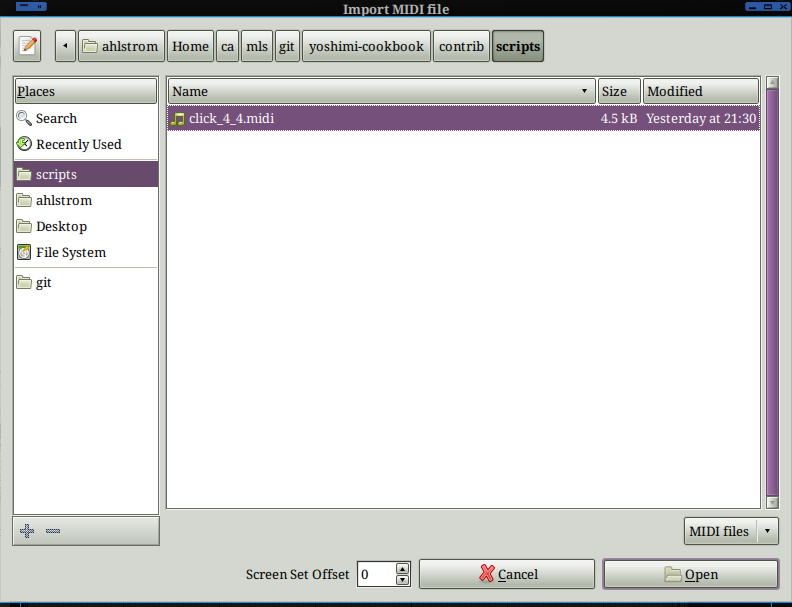
\includegraphics[scale=0.5]{menu/menu_file_import.png}
   \caption{Import MIDI}
   \label{fig:seq64_midi_export_file_import}
\end{figure}

   When imported, each track, whether a music track or an information track,
   is entered into its own loop/pattern box (slot).  The import operation can
   handle reasonably complex files.
%  as shown in the following diagram, which shows an import of
%  such as the \texttt{contrib/b4uacuse.mid} file, which contains
%  a transcription of an Eric Clapton / Robert Cray tune made over 20 years ago.
%  and had uploaded to the \textsl{GEnie} network service.

   Note the additional file-dialog field,
   \textbf{Select Screen Offset}.
   This field is present only in Gtkmm, but not Qt; in Qt, the current
   selected screen-set/bank is where the import is loaded, and the patterns
   are appended after any existing patterns.
   \index{import!select screen offset}
   \index{select screen offset}
   This setting is actually a set offset.
   It lets one place the imported data into a screen-set other than
   the first screen-set (screen-set 0).
   This field is not editable.  It requires using the scroll button to move the
   screen set offset up or down in value, from 0 to 31.

   When the file is imported, the sequence number for each track read is
   adjusted to put the track in the desired screen-set.
   The import can place the imported data into any of the 32 available
   screen-sets.  Quite large songs can be built by importing patterns.

   Import also handles SMF 0 MIDI files.  It parcels out the SMF 0 data
   into sequences/patterns for each of the 16 MIDI channels.  It also puts
   all of the MIDI data into the 17th pattern (pattern 16), in case it is
   needed.  Note that this slot is used no matter which screen-set one imports
   the file into.  Bug, or feature?

\subsection{Export Song as MIDI}
\label{subsec:seq64_midi_export_file_export}

   Thanks to the \textsl{Seq32} project, the ability to export songs to MIDI
   format has been added.
   "But wait!", you say, "Sequencer64 already saves to a MIDI-compatible
   format.  Why the need for an Export operation?"
   Well, the \textbf{Export Song as MIDI} operation modifies the song in the
   following ways:

   \begin{itemize}
      \item Only tracks (sequences, loops, or patterns)
         \index{exportable}
         that are "exportable" are written.  To be exportable, a
         track must be unmuted, and it must have triggers (see
         \sectionref{subsubsec:concepts_terms_trigger}).  That is,
         the track must have a layout entry in the \textbf{Song Editor}.
         A track need not have any playable data to be exported.
      \item All of the triggers for a given track are consolidated.  Each
         trigger generates the events, including repeats and
         offset-play of the track information.
         If there is a gap in the layout (e.g.
         due to an \textbf{Expand} operation in the Song Editor), then the
         corresponding gap in the events is exported. The result is
         a track that reconstructs the original
         playback/performance layout of that pattern.
%        This track is not needed (or even usable) in any
%        non-Seq24-based MIDI sequencer;
         The events themselves are sufficient to play the performance exactly.
         The triggers are useful
         for further editing of the song/performance,
         so they are preserved (in a \textbf{SeqSpec} section).
      \item Any empty pattern slots between tracks are removed.
      \item No matter what set the original track was in, it ends up in the
         first set.
      \item Other additions, such as time signature and tempo meta events, are
         written in the same manner as for a normal \textbf{File / Save}
         operation.
   \end{itemize}

\begin{figure}[H]
   \centering 
   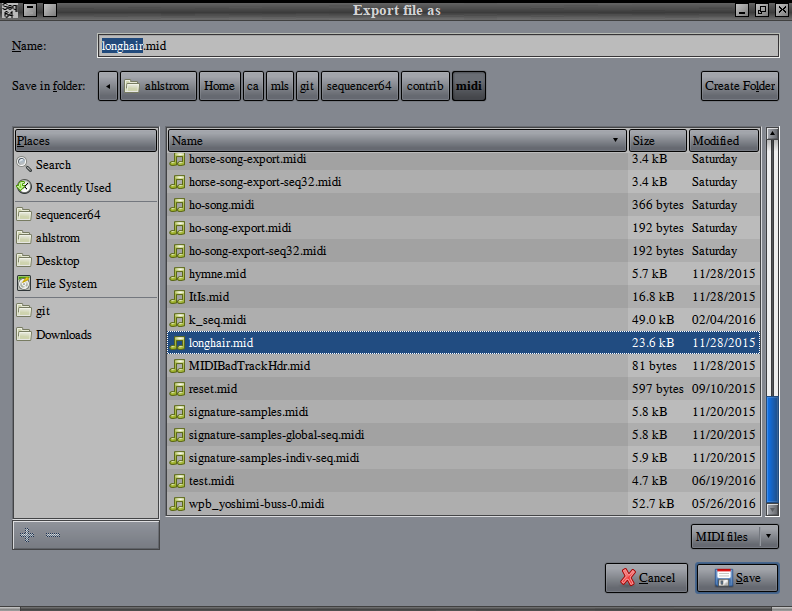
\includegraphics[scale=0.5]{menu/menu_file_export.png}
   \caption{File / Export Song as MIDI}
   \label{fig:seq64_midi_export_file_export}
\end{figure}

   If there are no exportable tracks, the following message is shown:

\begin{figure}[H]
   \centering 
   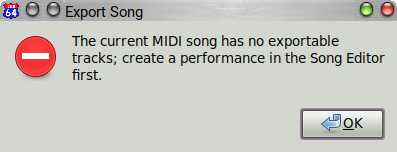
\includegraphics[scale=0.75]{menu/menu_file_unexportable.png}
   \caption{Unexportable MIDI File}
   \label{fig:seq64_midi_export_file_unexportable}
\end{figure}

   Once the file is exported, open it to see
   the results of the export.  Both the main window and the
   song performance window show the results of the export.
   Here is a short song, in two sets, shown in a composite view of four windows,
   showing each set and the performance layout of the tracks in the sets.
   (Note the second Song Editor window.)

\begin{figure}[H]
   \centering 
   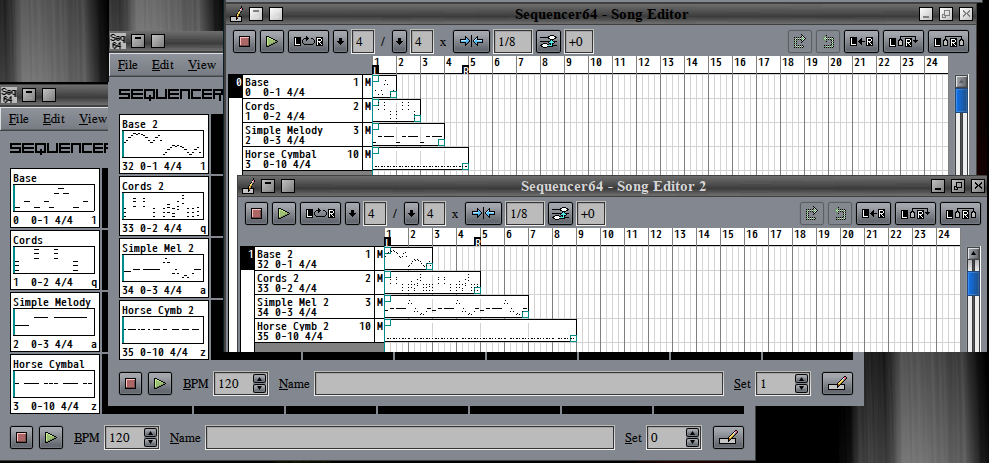
\includegraphics[scale=0.50]{export/original-song-to-export.png}
   \caption{Composite View of an Exportable Song}
   \label{fig:seq64_original_song_to_export}
\end{figure}

   The left column shows the four tracks of the first set (Set 0), the next
   column shows the four tracks of the second set (Set 1), and the
   layouts of the two sets are shown in the remainder of the diagram.
   Export this song, and see the result:

\begin{figure}[H]
   \centering 
   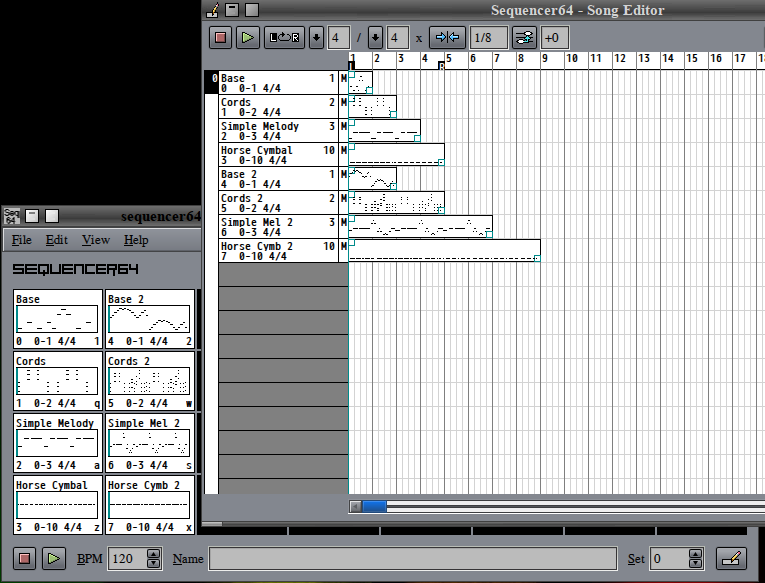
\includegraphics[scale=0.75]{export/song-exported.png}
   \caption{Composite View of Exported Song}
   \label{fig:seq64_song_exported}
\end{figure}

   One sees that the two sets are now combined into the first set,
   and all of the track layouts (triggers) have been exported.
   Had there been gaps in layouts or repeats of layouts in the song/performance
   data, these would have been reflected in the triggers.
   Much more complex examples are possible.

\subsection{Export MIDI Only}
\label{subsec:seq64_midi_export_file_export_midi_only}

   Sometimes it might be useful to export only the non-sequencer-specific
   (non-SeqSpec) data from a \textsl{Sequencer64} song.
   For example, some buggy sequencers
   (hello \textsl{Windows Media Player})
   might balk at some SeqSpec item in the song, and refuse to load the MIDI
   file.
   For such cases,
   the \textbf{Export MIDI Only} menu item writes a file that does not contain
   the SeqSpec data for each track, and does not include all the SeqSpec data
   (such as mute groups) that is normally written to the end of the
   \textsl{Sequencer64} MIDI file.
   Note that the meta data for track name is still written, so that the
   resulting file might be a little larger than the original
   \texttt{.mid} file that was imported into \textsl{Sequencer64}.

%  Also note that other meta data not handled by \textsl{Sequencer64},
%  such as Meta \texttt{FF 21 01 pp} (MIDI port pp), are also lost.

%-------------------------------------------------------------------------------
% vim: ts=3 sw=3 et ft=tex
%-------------------------------------------------------------------------------
